\section{Implementation}

Groovy was chosen as a language for implementation for two reasons, firstly it has a very efficient web framework called Grails built on the Spring framework, which is not only proven to be very robust and scalable, but is also very easy to implement and so enables quick agile development cycles. Previous implementations using Java/Spring and Java/Roo have proved very time-consuming to experiment with, whereas Grails has proven to be more flexible and easier to experiment with. The Groovy language also offers both some functional capability, as well as dynamic meta-programming capability. Domain specific languages (DSL’s) can be easily built on this framework, and this capability offers some scope to build a DSL based on the DataMOF ideas expanded in the previous section.
 
The Model Catalogue implementation discussed here has been implemented by building a core Models Catalogue based around these ideas using Groovy within the Grails framework. Some consideration was given to using the EMF/ECore framework, however the Grails framework offered a robust web-based alternative, with enough Model-Driven capability to test out the core ideas expressed here using a maintainable java-based stack that could be worked on by mainstream developers without a detailed knowledge of EMF. 

The front end user interface was implemented using a combination of HTML with javascript and CSS, the principal framework used being Angular JS. Communication with the client was carried out using a REST controller, enabling a variety of clients potentially to link up with the Model Catalogue.

GORM was used as a persistence mechanism, with a MySQL relational database as storage, although different GORM adapters made it possible to attach NO SQL datastores such as Neo4J and MongoDB. The full architectural stack is shown in figure\ref{fig:ApplicationArchitectMDR}


\begin{figure}[here]
	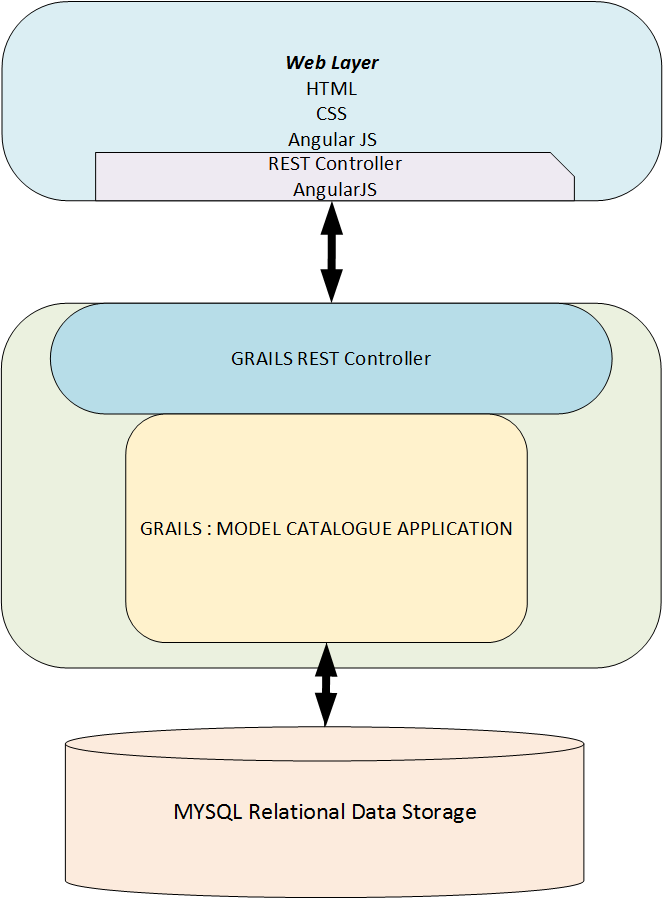
\includegraphics[width=0.5\textwidth,natwidth=610,natheight=642]{ApplicationArchitect1}
	\caption{Overview Architecture} 
	\label{fig:ApplicationArchitectMDR}
\end{figure}



 
 